\section[The Cosmic Microwave Background]{\hyperlink{toc}{The Cosmic Microwave Background}}

\subsection{Baryon-to-Photon Ratio and Recombination Temperature}
We recall the fractional ionization as solved for using the Saha equation:
\begin{equation}
    X = \frac{-1 + \sqrt{1 + 4S}}{2S}
\end{equation}
where $S$ is given by:
\begin{equation}
    S(T, \eta) = 3.84\eta\left(\frac{kT}{m_e c^2}\right)^{3/2}\exp(\frac{Q}{kT})
\end{equation}
where $T$ is the temperature, $\eta$ is the baryon-to-photon ratio, and $Q$ is the ionization energy. We take $k = 8.62 \times 10^{-5}\si{eV.K^{-1}}$, $Q = 13.6\si{eV}$, $m_e c^2 = 511000\si{eV}$. For $\eta = 4 \times 10^{-10}$ and for $\eta = 8 \times 10^{-10}$, we get:
\begin{figure}[htbp]
    \centering
    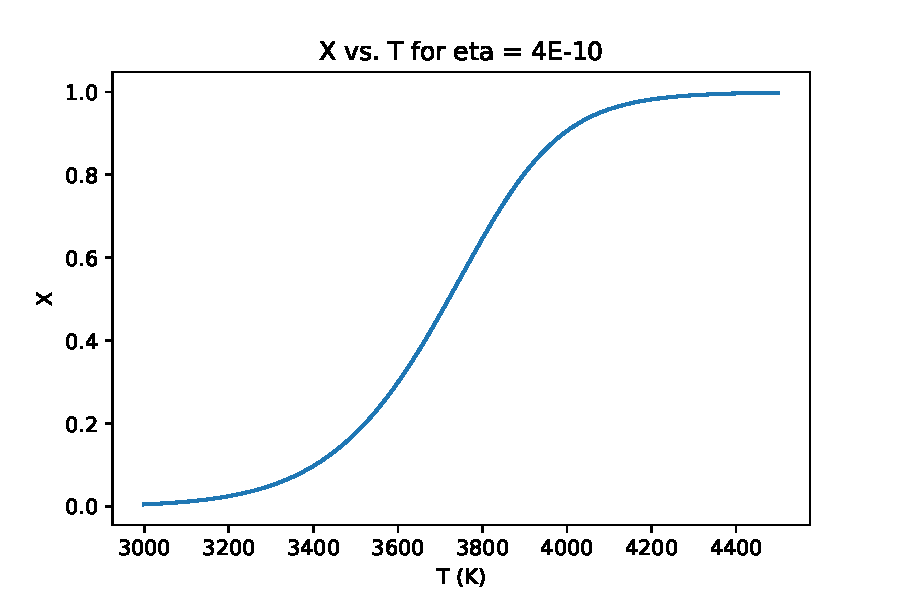
\includegraphics[scale=0.52]{Images/Q8-1eta4.pdf}
    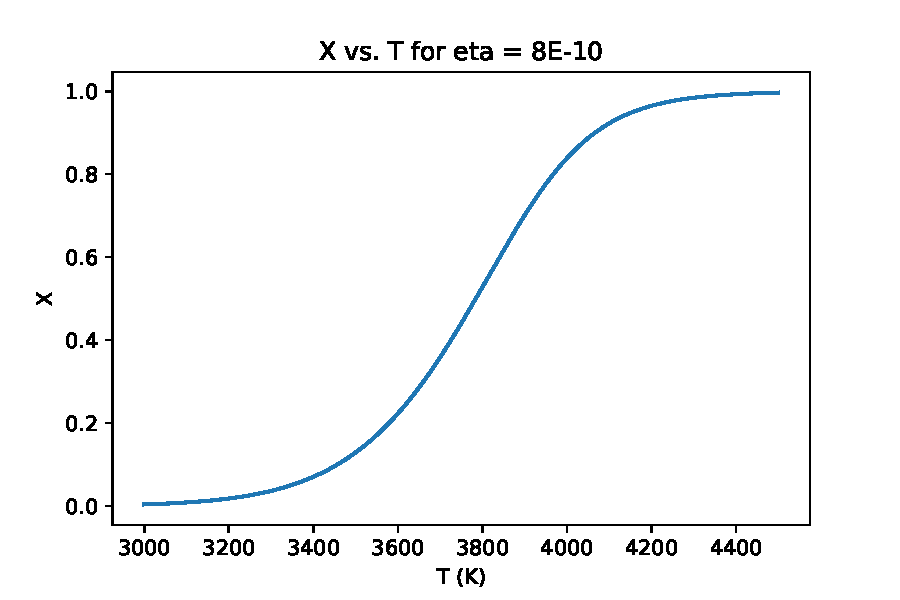
\includegraphics[scale=0.52]{Images/Q8-1eta8.pdf}
    
    \caption{Plots of fractional ionization $X$ as a function of temperature $T$ (in Kelvin) for baryon-to-photon ratios $\eta = 4 \times 10^{-10}$ and $\eta = 8 \times 10^{-10}$.}
    \label{fig-Q81}
\end{figure}

Taking $T_{\text{rec}}$ to be when $X = 1/2$, for $\eta = 4 \times 10^{-10}$, we have $\boxed{T_{\text{rec}} = 3720\si{K}}$, and for $\eta = 8 \times 10^{-10}$, we have $\boxed{T_{\text{rec}} = 3784\si{K}}$. Doubling the photon-to-baryon ratio has a small effect (only a relative change of about $1.7\%$).

\subsection{An ionizing photon per baryon}
From Problem 2.5, we recall:
\begin{equation}
    \frac{n(hf > E_0)}{n_\gamma} \approx 0.42\left(\frac{E_0}{kT}\right)^2\exp(-\frac{E_0}{kT})
\end{equation}
So setting $n(hf > E_0) = n_{\text{bary}}$ to have 1 ionizing photon per baryon, and letting $E_0 = Q$, we find:
\begin{equation}
    \eta = \frac{n_{\text{bary}}}{n_{\gamma}} = \frac{n(hf > Q)}{n_\gamma} = 0.42\left(\frac{Q}{kT}\right)^2\exp(-\frac{Q}{kT})
\end{equation}
With $Q = 13.6\si{eV}$ and $\eta = 6.1 \times 10^{-10}$, we can numerically solve the above relation to find:
\begin{equation}
    \boxed{T = 5823\si{K}}
\end{equation}
which is larger than the recombination temperature.

\subsection{Completely Helium at Recombination}
We start with Ryden Eq. 8.28:
\begin{equation}
    \frac{n_H}{n_pn_e} = \frac{g_H}{g_pg_E}\left(\frac{m_H}{m_p m_e}\right)^{3/2}\left(\frac{kT}{2\pi \hbar^2}\right)^{-3/2}\exp(\frac{[m_p + m_e - m_H]c^2}{kT}) =  \frac{g_H}{g_pg_E}\left(\frac{m_H}{m_p m_e}\right)^{3/2}\left(\frac{kT}{2\pi \hbar^2}\right)^{-3/2}\exp(\frac{Q_H}{kT})
\end{equation}
The analogous relation for the Helium atom is:
\begin{equation}
    \frac{n_{He}}{n_en_{He^+}} = \frac{g_{He}}{g_eg_{He^+}}\left(\frac{m_{He}}{m_e m_{He^+}}\right)^{3/2}\left(\frac{kT}{2\pi \hbar^2}\right)^{-3/2}\exp(\frac{Q_{He}}{kT})
\end{equation}
Using that the statistical factor is $g_{He}/g_eg_{He^+} = 1/4$ and that $m_{He} \sim m_{He^+} \sim 4m_p$, this becomes:
\begin{equation}
    \frac{n_{He}}{n_en_{He^+}} = \frac{1}{4}\left(\frac{m_e k T}{2\pi \hbar^2}\right)^{-3/2}\exp(\frac{Q_{He}}{kT})
\end{equation}
Defining $X = \frac{n_{He^+}}{n_{He^+} + n_{He}}$, we have that:
\begin{equation}
    n_{He} = \frac{1 - X}{X}n_{He^+}
\end{equation}
and from charge neutrality, $n_{He^+} = n_e$, so:
\begin{equation}\label{temp83}
    \frac{1 - X}{X} = n_{He^+}\frac{1}{4}\left(\frac{m_e kT}{2\pi \hbar^2}\right)^{-3/2}\exp(\frac{Q_{He}}{kT})
\end{equation}
If the Baryonic portion of the universe consists entirely of Helium-4 at the time of recombination, we then have that:
\begin{equation}
    \eta = \frac{4n_{He^+}}{X n_\gamma}
\end{equation}
Noting the $4$ as there are four baryons per Helium nucleus. Therefore using the blackbody number density of photons (Ryden Eq. 8.23):
\begin{equation}
    n_{He^+} = 0.2436\frac{X}{4}\eta\left(\frac{kT}{\hbar c}\right)^{3}
\end{equation}
And plugging this back into \eqref{temp83}, we have:
\begin{equation}
    \frac{1 - X}{X^2} = \frac{3.84}{16}\eta\left(\frac{kT}{m_e c^2}\right)^{3/2}\exp(\frac{Q_{He}}{kT})
\end{equation}
We now solve for the time of recombination. Setting $X = 1/2$, we have:
\begin{equation}
    2 = \frac{3.84}{16}\eta\left(\frac{kT_{\text{rec}}}{m_e c^2}\right)^{3/2}\exp(\frac{Q_{He}}{kT_{\text{rec}}})
\end{equation}
We now take $\eta = 6 \times 10^{-10}$ and $Q_{He} = 24.6\si{eV}$, and substitute in the standard values for the other constants. We can then umerically solve for $T_{\text{rec}}$ to get:
\begin{equation}
    \boxed{T_{\text{rec}} = 6490\si{K}}
\end{equation}

\subsection{Distances to Last Scattering}
From Fig 5.9, we can see that at $z_{\text{ls}} = 1090$, the propert distance approaches its limiting value of $3.20c/H_0$, so:
\begin{equation}
    \boxed{d_{\text{p, ls}} = 3.20\frac{c}{H_0} = 14000\si{Mpc}}.
\end{equation}
Finding the luminosity distance is then just multiplying the above by a factor of $(1 + z_{\text{ls}})$:
\begin{equation}
    \boxed{d_{\text{L, ls}} = (1 + z_{\text{ls}})d_{\text{p, ls}} = 1091d_{\text{p, ls}} = 15274\si{Gpc}}.
\end{equation}